\documentclass[12pt,a4paper]{article}
\usepackage[utf8]{inputenc}
\usepackage[T1]{fontenc}
\usepackage[english]{babel}
% Use Latin Modern scalable fonts to avoid PK bitmap font generation on MiKTeX
\usepackage{lmodern}
% Provide text-mode micro symbol if needed and other text symbols
\usepackage{textcomp}
\usepackage{graphicx}
\usepackage{amsmath}
\usepackage{amsfonts}
\usepackage{amssymb}
\usepackage{booktabs}
\usepackage{multirow}
\usepackage{longtable}
\usepackage{array}
\usepackage{xcolor}
\usepackage{colortbl}
\usepackage{float}
\usepackage{placeins}
\usepackage{caption}
\usepackage{subcaption}
\usepackage{geometry}
\usepackage{microtype} % Added for better text justification
\usepackage{ragged2e}  % Added for better text control
\usepackage{setspace}
\usepackage{titlesec}
\usepackage{enumitem}
\usepackage{siunitx}
\usepackage{tikz}
\usepackage{pgfplots}
\pgfplotsset{compat=1.18}
\usetikzlibrary{patterns}
\usepackage{hyperref}
\usepackage{cleveref}
\usepackage{fancyhdr}
\geometry{a4paper, margin=1in}

% Professional styling
\definecolor{LinkBlue}{HTML}{0B3C5D}
\definecolor{AccentGray}{HTML}{4F4F4F}
\hypersetup{
    colorlinks=true,
    linkcolor=LinkBlue,
    citecolor=LinkBlue,
    urlcolor=LinkBlue,
    pdfauthor={José Afonso da Silva Domingues de Moura, João Nuno Souteiro Bugalho Coelho},
    pdftitle={Breast Cancer Classification Using Clinical Biomarkers}
}
\captionsetup{
    font=small,
    labelfont=bf,
    labelsep=period
}
\setstretch{1.1}
\setlength{\parskip}{0.6em}
\setlength{\parindent}{0pt}
\setlength{\headheight}{14pt}
\setlist[itemize]{leftmargin=1.2em, topsep=0.3em, itemsep=0.1em}
\setlist[enumerate]{leftmargin=1.2em, topsep=0.3em, itemsep=0.1em}
\sisetup{detect-all=true}
\titleformat{\section}{\normalfont\Large\bfseries\color{AccentGray}}{\thesection}{0.6em}{}
\titleformat{\subsection}{\normalfont\large\bfseries\color{AccentGray}}{\thesubsection}{0.6em}{}
\titlespacing*{\section}{0pt}{1.4em}{0.7em}
\titlespacing*{\subsection}{0pt}{1em}{0.5em}
\titlespacing*{\subsubsection}{0pt}{0.8em}{0.4em}
\pagestyle{fancy}
\fancyhf{}
\fancyhead[LE,RO]{\thepage}
\fancyhead[LO]{Breast Cancer Biomarkers}
\fancyhead[RE]{Domingues de Moura \& Coelho}
\renewcommand{\headrulewidth}{0.4pt}
\renewcommand{\footrulewidth}{0pt}

\title{Breast Cancer Classification Using Clinical Biomarkers: \\ Applying Machine Learning Techniques for Feature Selection and Dimensionality Reduction}
\author{José Afonso da Silva Domingues de Moura (2021273987)\\
João Nuno Souteiro Bugalho Coelho	 (2021275030)}
\date{\today}

\begin{document}

\justifying

\maketitle

\newpage
\tableofcontents
\vspace{1em}
\hrule
\vspace{1em}
\newpage

\begin{abstract}
Breast cancer remains one of the most prevalent malignancies affecting women worldwide, with early detection being critical for treatment success. This study presents a comprehensive evaluation of machine learning techniques for breast cancer classification using blood-based clinical biomarkers from 116 patients. We systematically compare feature selection methodologies—including Kruskal-Wallis ranking, ROC-AUC analysis, and correlation-based selection—alongside dimensionality reduction techniques (PCA and LDA) across seven classifier families: Minimum Distance, Fisher LDA, Gaussian Bayes, K-Nearest Neighbors, Support Vector Machines, Decision Trees, AdaBoost, and Random Forest. Through Monte Carlo cross-validation, our analysis assessed various classification methods. The SVM classifier with RBF kernel attained the highest discriminative ability (ROC-AUC: 0.870, F1-Score: 0.816, Sensitivity: 0.804, Specificity: 0.814), demonstrating that targeted feature selection provides superior results compared to PCA's variance-based reduction. Glucose emerged as the single most discriminative biomarker (AUC: 0.800). These findings validate the potential of blood-based biomarkers as non-invasive screening tools and underscore the importance of statistical feature ranking over unsupervised methods for this classification task, offering practical pathways toward cost-effective early detection strategies in clinical settings.
\end{abstract}

\section{Introduction}
\label{sec:introduction}

Breast cancer remains one of the most prevalent malignancies affecting women worldwide, with early detection being crucial for successful treatment outcomes. The integration of machine learning techniques with clinical biomarker data offers promising avenues for improving diagnostic accuracy and risk assessment. This study leverages a dataset containing 116 patient records with various clinical parameters and biomarkers to develop an effective classification framework.

The analysis of blood-based biomarkers presents a less invasive alternative that could complement existing screening methods. This research systematically evaluates multiple feature selection strategies to identify the most predictive biomarkers for breast cancer classification.

This work builds upon a previous study \cite{patricio2018using} that explored similar concepts, with the same dataset and classification problem. However, in this report, we focus more on the feature selection and dimensionality reduction aspects, while also implementing some classifiers to validate the selected features. The differences on the main classification results presented here compared to the previous study will be discussed at the end of the Results section.


\section{Methodology}
\label{sec:methodology}

\subsection{Dataset Description}
\label{subsec:dataset}

The dataset comprises 116 patient records with the following features:

\begin{itemize}
    \item \textbf{Demographic Features:}
    \begin{itemize}
        \item Age (years)
        \item BMI (Body Mass Index)
    \end{itemize}
    
    \item \textbf{Blood Biomarkers:}
    \begin{itemize}
        \item Glucose (mg/dL)
        \item Insulin ($\mu$U/mL)
        \item HOMA (Homeostatic Model Assessment)
        \item Leptin (ng/mL)
        \item Adiponectin ($\mu$g/mL)
        \item Resistin (ng/mL)
        \item MCP-1 (pg/mL)
    \end{itemize}
    
    \item \textbf{Target Variable:}
    \begin{itemize}
        \item Classification (1: Healthy, 2: Breast Cancer)
    \end{itemize}
\end{itemize}

\subsection{Data Preprocessing}
\label{subsec:preprocessing}

The data preprocessing pipeline included the following steps:

\subsubsection{Data Partitioning}
The dataset was split into training and testing sets using a 70-30 split ratio:
\begin{itemize}
    \item Training set: 81 samples
    \item Test set: 35 samples
\end{itemize}

\subsubsection{Feature Normalization}
All features were standardized using z-score normalization:
\[
x_{\text{normalized}} = \frac{x - \mu}{\sigma}
\]
where $\mu$ represents the mean and $\sigma$ represents the standard deviation of each feature in the training set.

To prevent data leakage and ensure the test set remains independent, normalization parameters were computed solely from the training data and applied to both training and test sets.

\subsection{Feature Selection Methods}
\label{subsec:feature_selection}

\subsubsection{Kruskal-Wallis Test}
The Kruskal-Wallis non-parametric test was employed to assess feature importance. It evaluates whether the distribution of a feature differs significantly between the two classes (healthy vs. breast cancer). Features were ranked based on their Kruskal-Wallis statistic values, where higher values indicate greater discriminatory power. 


\subsubsection{ROC-AUC Analysis}
Receiver Operating Characteristic (ROC) analysis was performed for each feature individually, with Area Under Curve (AUC). The AUC shows the ability to discriminate between classes, derived from the relationship between the true positive rate (TPR) and false positive rate (FPR).
Features were ranked based on their AUC scores, with higher scores indicating better discriminative power.

% Show ROC curves
\begin{figure}[H]
  \centering
  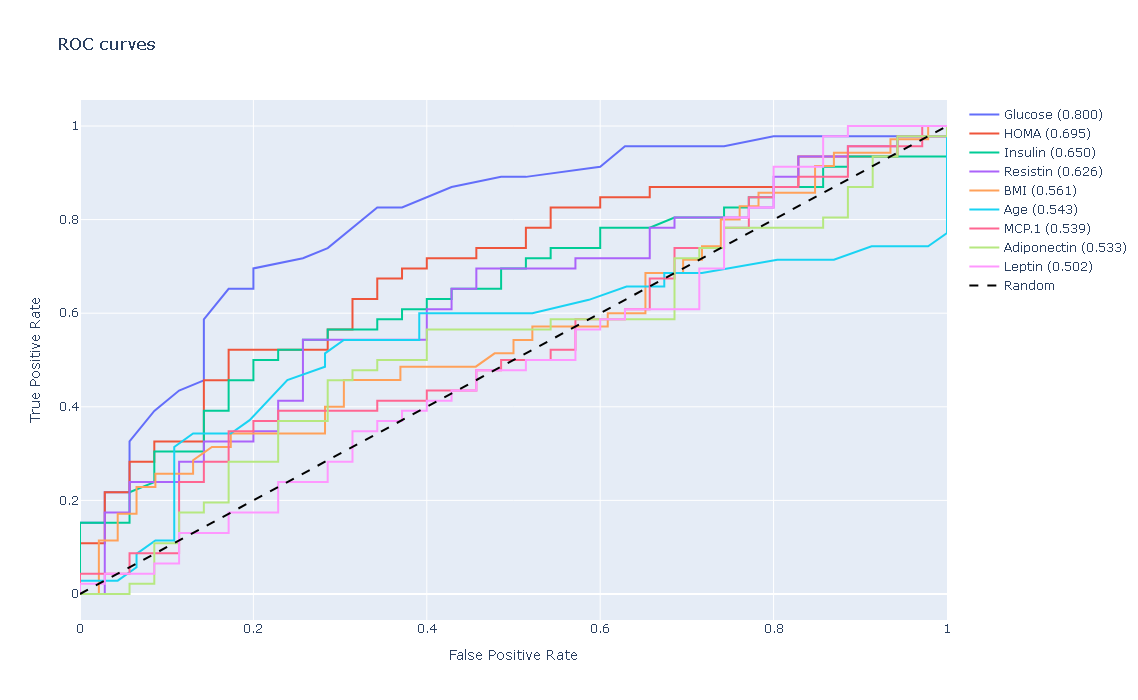
\includegraphics[width=0.8\textwidth]{imgs/plt_roc_curves.png}
  \caption{ROC curves for each feature}
  \label{fig:roc_curves}
\end{figure}
 

\subsubsection{Correlation-based Feature Selection}
A threshold-based approach was implemented to select features based on their correlations with the other features. Priority is given to features that show higher correlation with the target variable (Classification). However, highly correlated features among themselves should be avoided to reduce redundancy. 

To achieve this, a correlation matrix was initially computed, followed by the sorting of features based on their absolute correlation with the target variable. For each one of these, another check was made to see if its correlation with any other feature was above a predefined threshold (0.90). If so, the the lower-ranked feature is discarded to reduce redundancy.

\begin{figure}[H]
  \centering
  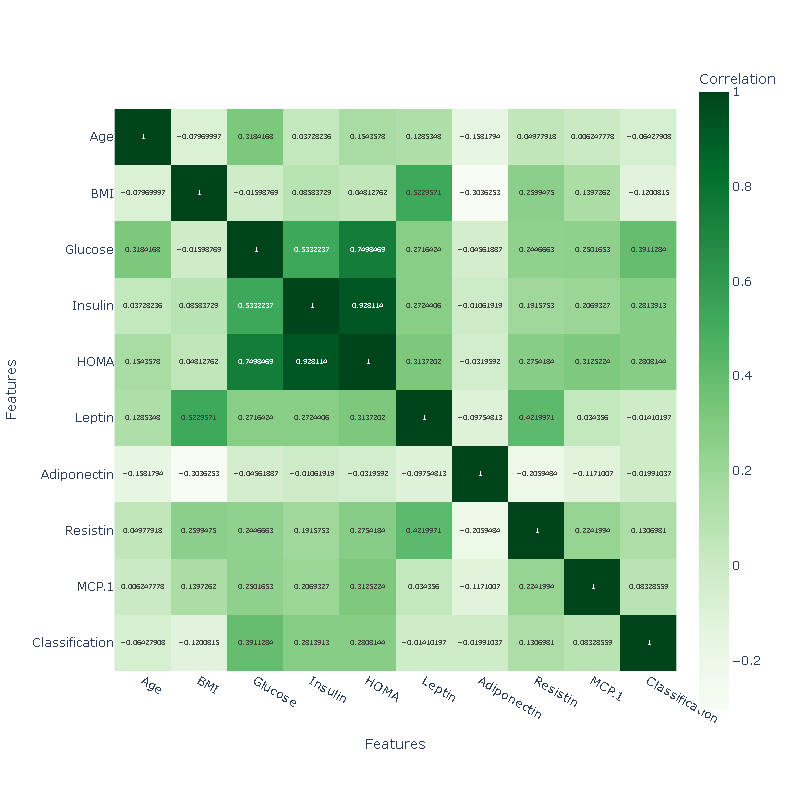
\includegraphics[width=0.6\textwidth]{imgs/correlation_heatmap.png}
  \caption{Correlation matrix heatmap of features including the target variable}
  \label{fig:correlation}
\end{figure}
\FloatBarrier

As it can be seen in Figure~\ref{fig:correlation}, there is a pair of features which are highly correlated (Insulin and HOMA). Given that HOMA has a higher correlation with the target variable, Insulin was discarded in this step.

This process was also done using only data from the training set.

\subsection{Dimensionality Reduction}
\label{subsec:dim_reduction}

\subsubsection{Principal Component Analysis (PCA)}
PCA was applied to transform the original feature space into a lower-dimensional representation in an unsupervised manner. For this, the PCA object from the \texttt{sklearn.decomposition} library was used, retaining components that explained a significant portion of the variance. Similar to the normalization step, PCA was fitted on the training data and then applied to both training and test sets (fitting PCA on the training set also helps detect overfitting). Therefore, two functions were developed: one to fit the PCA on the training set and another to apply the fitted PCA to any other set (training or test).

\subsubsection{Linear Discriminant Analysis (LDA)}
LDA was employed as a supervised dimensionality reduction technique to maximize class separability. The LDA model from the \texttt{sklearn.discriminant\_analysis} library was fitted on the training data, and the resulting transformation was applied to both training and test sets. Given that LDA can produce at most (C-1) components, where C is the number of classes, in this binary classification problem, LDA reduced the feature space to a single dimension.

\subsection{Classification Models}
\label{subsec:classification_models}
Several classification algorithms were implemented to evaluate the effectiveness on predicting breast cancer basedon the features that were given. The following classifiers were explored using a Monte Carlo Cross-Validation (MCCV) approach with 150 iterations, where in each iteration the dataset is randomly split into training and test sets (70-30 split). The average performance metrics across all iterations were computed to assess the classifiers' effectiveness. Metrics taken into account include sensitivity, specificity, precision, F1-score and ROC-AUC.

\subsubsection{Minimum Distance classifiers}
Minimum Distance classifiers were implemented to classify samples based on their proximity to class centroids in the feature space. Two different distance metrics were explored: Euclidean distance and Mahalanobis distance. While the Euclidean distance is the straight-line distance between two points, the Mahalanobis distance accounts for the correlations between features, usually providing a more accurate measure of distance in cases where features are correlated. Classification decisions were made by assigning each sample to the class of the nearest centroid. For this purpose, the \texttt{minimum\_distance\_classifier} was developed in order to store centroids and compute distances based on the selected metric and make predictions. The classifier was trained on the training set and evaluated on both training and test sets in order to evaluate performance and potential overfitting.


\subsubsection{Fisher's Linear Discriminant Analysis (LDA) Classifier}
Fisher's LDA was utilized to find a linear combination of features that best separates the classes. The LDA model from the \texttt{sklearn.discriminant\_analysis} library was fitted on the training data, and the resulting transformation was applied to both training and test sets. However, it is known that, for only two classes, this classifier is equivalent to a Minimum Distance classifier with Mahalanobis distance. Explanation is given in the Results section.

\subsubsection{Bayes Classifier}
A Gaussian classifier assumes that each class follows a multivariate normal distribution and combines the class-conditional likelihood with the prior probability of each class. In our implementation, we estimate one Gaussian per class (mean, full covariance, and empirical prior), then apply Bayes rule to compute posterior probabilities and pick the class with the highest posterior. This approach models the joint distribution directly, which can capture feature correlations but may be sensitive to poorly estimated covariances when data is limited. In this case, tests were run using different combinations of features, including all features, top features from Kruskal-Wallis ranking and top features from ROC-AUC ranking. 

\subsubsection{KNN Classifier}
The K-Nearest Neighbors (KNN) classifier was implemented to classify samples based on the majority class among their k-nearest neighbors in the feature space. Various values of k were tested, along with different distance metrics (Euclidean, Manhattan, and Minkowski) and weighting schemes (uniform and distance-based). The \texttt{KNeighborsClassifier} from the \texttt{sklearn.neighbors} library was used for this purpose. The classifier was trained on the training set and evaluated on both training and test sets to assess performance and potential overfitting.

\subsubsection{SVM Classifier}
Support Vector Machine (SVM) classifiers were employed to find the optimal hyperplane that separates the classes in the feature space. Both linear and non-linear kernels (e.g., radial basis function) were explored to capture complex decision boundaries. The \texttt{SVC} class from the \texttt{sklearn.svm} library was utilized for this purpose. The classifier was trained on the training set and evaluated on test sets to assess performance.

\subsubsection{Decision Tree Classifier}
Decision Tree classifiers were implemented using the \texttt{DecisionTreeClassifier} from the \texttt{sklearn.tree} library. Various hyperparameter configurations were tested, including criterion type, maximum depth, and minimum samples constraints, to optimize the balance between model complexity and generalization.

\subsubsection{AdaBoost Classifier}
AdaBoost (Adaptive Boosting) was employed as an ensemble method to combine multiple weak learners (shallow decision trees) into a robust classifier. The algorithm iteratively trains decision trees with limited depth and adjusts sample weights to focus on misclassified instances. Each weak learner is assigned an alpha (confidence) coefficient based on its training accuracy. During prediction, the final decision is determined by aggregating weighted predictions across all weak learners. The \texttt{AdaBoostClassifier} was configured with varying numbers of estimators and tree depths to optimize the balance between bias and variance.

\section{Experimental Results}
\label{sec:results}

\subsection{Feature Selection Results}
\label{subsec:feature_results}

\subsubsection{Kruskal-Wallis Ranking}
The Kruskal-Wallis test revealed the following feature ranking:

\begin{table}[H]
\centering
\label{tab:kruskal}
        \begin{tabular}{@{}lc@{}}
            	\toprule
            	\textbf{Feature} & \textbf{Kruskal-Wallis Statistic} \\
\midrule
Glucose & 21.19 \\
HOMA & 8.96 \\
Insulin & 5.28 \\
Resistin & 3.75 \\
BMI & 0.89 \\
Age & 0.43 \\
MCP.1 & 0.35 \\
Adiponectin & 0.26 \\
Leptin & 0.001 \\
\bottomrule
\end{tabular}
\caption{Kruskal-Wallis Feature Ranking}
\end{table}

\subsubsection{ROC–AUC analysis}
The discriminatory power of each individual feature was assessed by computing Receiver Operating Characteristic (ROC) curves and the corresponding Area Under the Curve (AUC). For each feature, the ROC curve was constructed by comparing the continuous feature values against the binary class labels. For this, the \texttt{roc\_curve} and \texttt{auc} functions from the \texttt{sklearn.metrics} library were used.


% Combine ROC figure and AUC table side-by-side to save vertical space

\begin{table}[H]
    \centering
        \begin{tabular}{@{}lc@{}}
                \toprule
                \textbf{Feature} & \textbf{AUC Score} \\
            \midrule
            Glucose & 0.800 \\
            HOMA & 0.695 \\
            Insulin & 0.650 \\
            Resistin & 0.626 \\
            BMI & 0.561 \\
            Age & 0.543 \\
            MCP.1 & 0.539 \\
            Adiponectin & 0.533 \\
            Leptin & 0.502 \\
            \bottomrule
        \end{tabular}
        \caption{Feature AUC Scores}
        \label{tab:auc}
\end{table}

The results (Table~\ref{tab:auc}) indicate that Glucose exhibits the highest discriminative capability among the evaluated biomarkers (AUC = 0.800), followed by HOMA and Insulin, (consistent with the values presented in the correlation analysis, given that Insulin and HOMA are highly correlated). Features with AUC values close to 0.5 (e.g., Leptin) provide little to no discriminatory information on their own, exhibiting near-random behaviour. When having lower than 0.5, the true power of the feature is in the complementary value (1 - AUC), given that all that has to be done is to invert the predictions. These findings informed the subsequent feature selection and dimensionality reduction stages: features with superior AUC were prioritized when constructing reduced feature sets.

\subsubsection{Correlation Analysis}
The correlation matrix heatmap (Figure~\ref{fig:correlation}) revealed moderate correlations between markers, though a pair of features was highly correlated (Insulin and HOMA). 

The "ranked" features based on their absolute correlation with the target variable were as follows:
\begin{table}[H]
\centering
        \begin{tabular}{@{}lc@{}}
            	\toprule
            	\textbf{Feature} & \textbf{Absolute Correlation with Target} \\
            \midrule
            Glucose & 0.391 \\
            Insulin & 0.281 \\
            HOMA & 0.280 \\
            Resistin & 0.131 \\
            BMI & 0.120 \\
            MCP & 0.083 \\
            Age & 0.064 \\
            Adiponectin & 0.019 \\
            Leptin & 0.014 \\
            \bottomrule
        \end{tabular}
\caption{Feature Ranking by Absolute Correlation with Target}
\end{table}

Again, Glucose stands out as the feature with the highest correlation with the target variable (0.391), followed by Insulin and HOMA. Given the high correlation between Insulin and HOMA, Insulin would be discarded to reduce redundancy.

\subsubsection{Feature Importance Analysis}
The consistent ranking of glucose as the most discriminative feature across multiple evaluation methods (Kruskal-Wallis: 21.19, AUC: 0.800) suggests a strong association between glucose metabolism and breast cancer risk.

The strong performance of HOMA (AUC: 0.695) and Insulin (AUC: 0.650) further supports the importance of metabolic health indicators in breast cancer classification. 

These results highlight the potential of using metabolic biomarkers as complementary tools in cancer diagnostic assessment.


\subsection{Dimensionality Reduction Results}

\subsubsection{PCA Results}
\label{subsec:pca_results}


After applying Principal Component Analysis (PCA) to the dataset containing nine original features, the following distribution of explained variance was obtained:
  
\begin{table}[H]
\centering
\begin{tabular}{ccc}
\toprule
\textbf{Component} & \textbf{Individual Variance} & \textbf{Cumulative Variance} \\
\midrule
PC1 & 33.74\% & 33.74\% \\
PC2 & 18.33\% & 52.07\% \\
PC3 & 12.51\% & 64.58\% \\
PC4 & 11.18\% & 75.77\% \\
PC5 & 8.68\% & 84.45\% \\
PC6 & 7.46\% & 91.91\% \\
PC7 & 4.32\% & 96.23\% \\
PC8 & 3.50\% & 99.74\% \\
PC9 & 0.26\% & 100.00\% \\
\bottomrule
\end{tabular}
\caption{Explained Variance by Principal Component}
\end{table}


\begin{figure}[H]
\centering
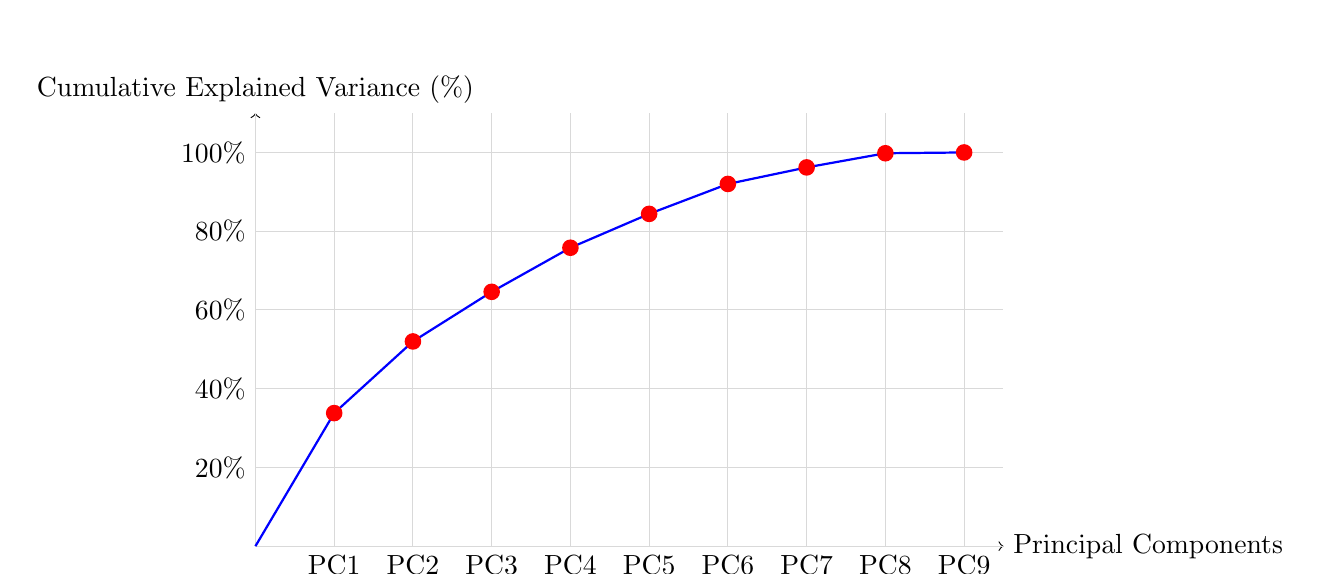
\begin{tikzpicture}
\draw[->] (0,0) -- (9.5,0) node[right] {Principal Components};
\draw[->] (0,0) -- (0,5.5) node[above] {Cumulative Explained Variance (\%)};

% Grid
\draw[gray!30] (0,0) grid (9.5,5.5);

% Data points (y = cumulative_percent / 20 to fit axis)
\coordinate (PC1) at (1,1.69);   % 33.74% -> 1.687
\coordinate (PC2) at (2,2.60);   % 52.07% -> 2.6035
\coordinate (PC3) at (3,3.23);   % 64.58% -> 3.229
\coordinate (PC4) at (4,3.79);   % 75.77% -> 3.7885
\coordinate (PC5) at (5,4.22);   % 84.45% -> 4.2225
\coordinate (PC6) at (6,4.60);   % 91.91% -> 4.5955
\coordinate (PC7) at (7,4.81);   % 96.23% -> 4.8115
\coordinate (PC8) at (8,4.99);   % 99.74% -> 4.987
\coordinate (PC9) at (9,5.00);   % 100.00% -> 5.00

% Plot line
\draw[blue, thick] (0,0) -- (PC1) -- (PC2) -- (PC3) -- (PC4) -- (PC5) -- (PC6) -- (PC7) -- (PC8) -- (PC9);

% Points
\foreach \point in {PC1,PC2,PC3,PC4,PC5,PC6,PC7,PC8,PC9} 
    \fill[red] (\point) circle (3pt);

% Labels (include PC9 now)
\node[below] at (1,0) {PC1};
\node[below] at (2,0) {PC2};
\node[below] at (3,0) {PC3};
\node[below] at (4,0) {PC4};
\node[below] at (5,0) {PC5};
\node[below] at (6,0) {PC6};
\node[below] at (7,0) {PC7};
\node[below] at (8,0) {PC8};
\node[below] at (9,0) {PC9};

% Y-axis labels (explicit percentages matching scale y*20)
\node[left] at (0,1) {20\%};
\node[left] at (0,2) {40\%};
\node[left] at (0,3) {60\%};
\node[left] at (0,4) {80\%};
\node[left] at (0,5) {100\%};
\end{tikzpicture}
\caption*{Evolution of cumulative explained variance by principal components}
\end{figure}

The first principal component explains approximately \textbf{33.7\%} of the total variance, while the first two components together account for about \textbf{52.1\%}. The first six components cumulatively explain around \textbf{91.9\%} of the total variance, indicating that reducing the dimensionality to six components would retain most of the original information.

The last components (particularly the eighth and ninth) contribute very little to the total variance, suggesting that they mostly capture noise or residual variability. Therefore, using between five and six components appears to provide a good balance between simplification and information retention.

\begin{figure}[H]
  \centering
  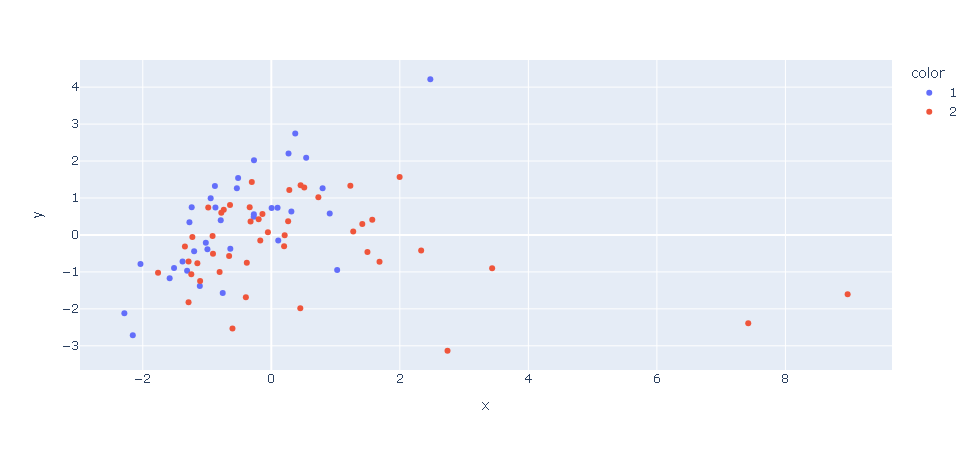
\includegraphics[width=0.8\textwidth]{imgs/pca_2d.png}
  \caption{Scatter with 2 most relevant PCA components on training set}
  \label{fig:pca_2d}
\end{figure}

\begin{figure}[H]
  \centering
  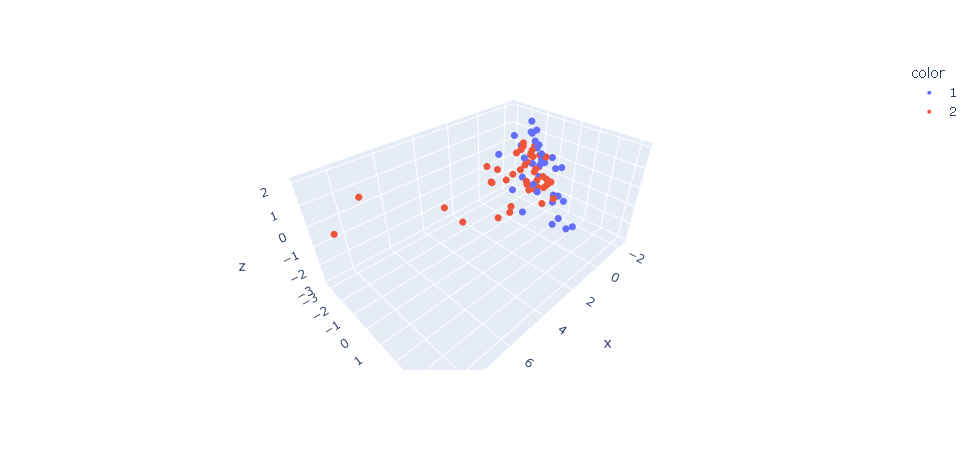
\includegraphics[width=0.9\textwidth]{imgs/pca_3d.png}
  \caption{Scatter with 3 most relevant PCA components on training set}
  \label{fig:pca_3d}
\end{figure}

\subsubsection{LDA Results}
LDA reduced the feature space to a single dimension, maximizing class separability compared to the PCA approach. This can be shown in the 1D scatter plot (Figure~\ref{fig:lda_1d}).

\begin{figure}[H]
  \centering
  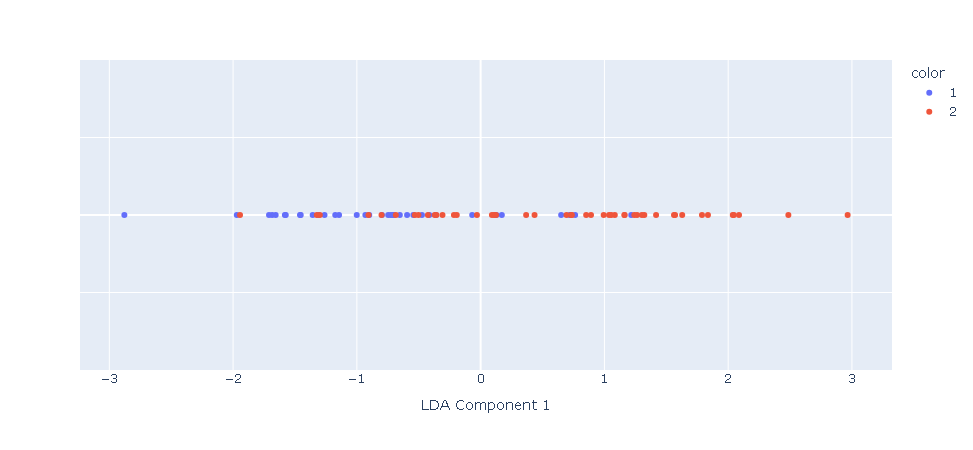
\includegraphics[width=0.8\textwidth]{imgs/lda_1d.png}
  \caption{1D scatter plot of LDA transformation on training set}
  \label{fig:lda_1d}
\end{figure}

This figure shows improved clustering compared to the PCA results, indicating effective dimensionality reduction, despite not being linearly separable.

\subsection{Classifier Results}
To ensure the robustness of the predictive models, a Monte Carlo Cross-Validation (MCCV) strategy was employed. The dataset was randomly partitioned into training (70\%) and testing (30\%) sets over 150 independent iterations ($N=150$). The performance metrics reported below represent the mean and standard deviation across these iterations, ensuring that the results account for data variability and minimize selection bias.
\label{subsec:classifier_results}

\subsubsection{Minimum Distance classifier}
The Minimum Distance classifier was evaluated using both Euclidean and Mahalanobis distance metrics. The performance performance metrics on the test set are summarized in Table~\ref{tab:euclidean_metrics} and Table~\ref{tab:mahalanobis_metrics}.

\subsubsection*{Classification Metrics Breakdown on Original Data}

\begin{table}[H]
    \centering
    \begin{tabular}{lc}
        \toprule
        \textbf{Metric} & \textbf{Value (Mean $\pm$ STD)} \\
        \midrule
        Sensitivity & $0.518 \pm 0.112$ \\
        Specificity & $0.811 \pm 0.101$ \\
        Precision   & $0.773 \pm 0.114$ \\
        F1-Score    & $0.612 \pm 0.096$ \\
        ROC-AUC     & $0.750 \pm 0.081$ \\
        \bottomrule
    \end{tabular}
    \caption{Performance metrics for the Minimum Distance classifier using \textbf{Euclidean Distance}.}
    \label{tab:euclidean_metrics}
\end{table}
\begin{table}[H]
    \centering
    \begin{tabular}{lc}
        \toprule
        \textbf{Metric} & \textbf{Value (Mean $\pm$ STD)} \\
        \midrule
        Sensitivity & $0.648 \pm 0.107$ \\
        Specificity & $0.761 \pm 0.124$ \\
        Precision   & $0.731 \pm 0.115$ \\
        F1-Score    & $0.697 \pm 0.085$ \\
        ROC-AUC     & $0.762 \pm 0.077$ \\
        \bottomrule
    \end{tabular}
    \caption{Performance metrics for the Minimum Distance Classifier using \textbf{Mahalanobis Distance}.}
    \label{tab:mahalanobis_metrics}
\end{table}

Comparing the two distance metrics, the Mahalanobis distance yields superior overall performance compared to the Euclidean distance, particularly regarding the balance between classes.

\begin{itemize}
    \item \textbf{Sensitivity vs. Specificity:} The Euclidean classifier (Table \ref{tab:euclidean_metrics}) exhibits a strong bias towards the negative class, resulting in high Specificity ($0.811$) but poor Sensitivity ($0.518$). In contrast, the Mahalanobis classifier (Table \ref{tab:mahalanobis_metrics}) significantly improves Sensitivity to $0.648$, albeit with a slight reduction in Specificity ($0.761$). This suggests that the Mahalanobis distance is more effective at identifying positive cases. Given that detecting breast cancer is critical, higher Sensitivity is often prioritized.
    
    \item \textbf{F1-Score:} The F1-Score, which represents the harmonic mean of precision and sensitivity, is notably higher for the Mahalanobis distance ($0.697$) compared to the Euclidean distance ($0.612$). This confirms that the Mahalanobis distance provides a better trade-off between false positives and false negatives.
    
    \item \textbf{ROC-AUC:} Both models demonstrate comparable discriminative ability across thresholds, with Mahalanobis ($0.762$) performing slightly better than Euclidean ($0.750$).
\end{itemize}


\subsubsection*{Minimum Distance classifier on Reduced Feature Sets}

This section evaluates the performance of the Minimum Distance classifier applied to feature sets transformed via Principal Component Analysis (PCA) and Linear Discriminant Analysis (LDA).

\subsubsection*{PCA Feature Reduction (Euclidean Distance)}

Table \ref{tab:pca_metrics} presents the classifier's performance as the number of Principal Components (PC) increases from 1 to 9.

\begin{table}[H]
    \centering
    \resizebox{\textwidth}{!}{
    \begin{tabular}{cccccc}
        \toprule
        \textbf{Components} & \textbf{Sensitivity} & \textbf{Specificity} & \textbf{Precision} & \textbf{F1-Score} & \textbf{ROC-AUC} \\
        \midrule
        1 & $0.496 \pm 0.111$ & $0.677 \pm 0.111$ & $0.655 \pm 0.102$ & $0.557 \pm 0.090$ & $0.647 \pm 0.083$ \\
        2 & $0.488 \pm 0.112$ & $0.757 \pm 0.114$ & $0.716 \pm 0.111$ & $0.571 \pm 0.093$ & $0.683 \pm 0.079$ \\
        3 & $0.496 \pm 0.110$ & $0.784 \pm 0.104$ & $0.741 \pm 0.108$ & $0.586 \pm 0.094$ & $0.707 \pm 0.079$ \\
        4 & $0.496 \pm 0.112$ & $0.774 \pm 0.106$ & $0.731 \pm 0.115$ & $0.583 \pm 0.100$ & $0.714 \pm 0.082$ \\
        5 & $0.494 \pm 0.119$ & $0.784 \pm 0.099$ & $0.738 \pm 0.113$ & $0.583 \pm 0.102$ & $0.726 \pm 0.083$ \\
        6 & $0.497 \pm 0.113$ & $0.804 \pm 0.099$ & $0.759 \pm 0.113$ & $0.592 \pm 0.097$ & $0.744 \pm 0.079$ \\
        7 & $0.519 \pm 0.113$ & $0.813 \pm 0.097$ & $0.775 \pm 0.110$ & $0.613 \pm 0.096$ & $0.752 \pm 0.081$ \\
        8 & $0.517 \pm 0.112$ & $0.813 \pm 0.101$ & $0.775 \pm 0.113$ & $0.612 \pm 0.095$ & $0.750 \pm 0.081$ \\
        9 & $0.518 \pm 0.112$ & $0.811 \pm 0.101$ & $0.773 \pm 0.114$ & $0.612 \pm 0.096$ & $0.750 \pm 0.081$ \\
        \bottomrule
    \end{tabular}
    }
    \caption{Performance of Minimum Distance classifier on \textbf{PCA-reduced data} (Mean $\pm$ STD).}
    \label{tab:pca_metrics}
\end{table}

\subsubsection*{PCA Feature Reduction (Mahalanobis Distance)}


\begin{table}[H]
    \centering
    \resizebox{\textwidth}{!}{
    \begin{tabular}{cccccc}
        \toprule
        \textbf{Components} & \textbf{Sensitivity} & \textbf{Specificity} & \textbf{Precision} & \textbf{F1-Score} & \textbf{ROC-AUC} \\
        \midrule
        1 & $0.496 \pm 0.111$ & $0.677 \pm 0.111$ & $0.655 \pm 0.102$ & $0.557 \pm 0.090$ & $0.647 \pm 0.083$ \\
        2 & $0.476 \pm 0.120$ & $0.749 \pm 0.113$ & $0.703 \pm 0.120$ & $0.558 \pm 0.104$ & $0.685 \pm 0.076$ \\
        3 & $0.517 \pm 0.125$ & $0.755 \pm 0.118$ & $0.727 \pm 0.112$ & $0.593 \pm 0.098$ & $0.712 \pm 0.079$ \\
        4 & $0.535 \pm 0.126$ & $0.726 \pm 0.130$ & $0.711 \pm 0.119$ & $0.598 \pm 0.095$ & $0.700 \pm 0.079$ \\
        5 & $0.584 \pm 0.131$ & $0.718 \pm 0.119$ & $0.719 \pm 0.112$ & $0.634 \pm 0.103$ & $0.714 \pm 0.083$ \\
        6 & $0.624 \pm 0.104$ & $0.751 \pm 0.133$ & $0.760 \pm 0.116$ & $0.676 \pm 0.079$ & $0.734 \pm 0.083$ \\
        7 & $0.626 \pm 0.096$ & $0.750 \pm 0.123$ & $0.758 \pm 0.112$ & $0.679 \pm 0.076$ & $0.741 \pm 0.083$ \\
        8 & $0.619 \pm 0.099$ & $0.736 \pm 0.130$ & $0.747 \pm 0.118$ & $0.669 \pm 0.081$ & $0.725 \pm 0.087$ \\
        9 & $0.648 \pm 0.107$ & $0.761 \pm 0.124$ & $0.771 \pm 0.115$ & $0.697 \pm 0.085$ & $0.762 \pm 0.077$ \\
        \bottomrule
    \end{tabular}
    }
    \caption{Performance of Minimum Distance classifier (Mahalanobis) on \textbf{PCA-reduced data} (Mean $\pm$ STD).}
    \label{tab:pca_mahalanobis_metrics}
\end{table}

\textbf{Note:} With Mahalanobis distance, performance improves steadily with more components; at 9 PCs the F1-Score ($0.697$) and Sensitivity ($0.648$) match the full-feature Mahalanobis baseline, showing that PCA retains the discriminative structure needed by the Mahalanobis metric.

\subsubsection*{LDA Feature Reduction}

Table \ref{tab:lda_metrics} shows the results obtained using the single component generated by LDA (using Euclidean or Mahalanobis distance gave similar results).

\begin{table}[H]
    \centering
    \begin{tabular}{lc}
        \toprule
        \textbf{Metric} & \textbf{Value (Mean $\pm$ STD)} \\
        \midrule
        Sensitivity & $0.497 \pm 0.131$ \\
        Specificity & $0.733 \pm 0.111$ \\
        Precision   & $0.695 \pm 0.116$ \\
        F1-Score    & $0.570 \pm 0.112$ \\
        ROC-AUC     & $0.697 \pm 0.083$ \\
        \bottomrule
    \end{tabular}
    \caption{Performance of Minimum Distance classifier on \textbf{LDA-reduced data}.}
    \label{tab:lda_metrics}
\end{table}


\begin{itemize}
    \item \textbf{PCA (Euclidean):} As components increase from 1 to 7–9, F1 rises from $0.557$ to $\approx 0.612$ and ROC-AUC reaches $0.750$, matching the full-space Euclidean baseline with 9 PCs. PCA preserves Euclidean structure, but Sensitivity stays modest ($\approx 0.52$).
    \item \textbf{PCA (Mahalanobis):} Adding Mahalanobis lifts Sensitivity and F1 monotonically; with 9 PCs, it reaches F1 $0.697$ and Sensitivity $0.648$, matching the full-feature Mahalanobis baseline. PCA retains the discriminative structure needed by the correlation-aware metric.
    \item \textbf{LDA 1D:} The supervised 1D projection attains F1 $0.570$ and ROC-AUC $0.697$, similar to PCA with 1–2 PCs, but below higher-dimensional PCA and well below PCA+Mahalanobis. The extreme 1D compression limits linear separability for the centroid classifier.
    \item \textbf{Class imbalance:} All variants show high Specificity ($>0.73$) and low-to-moderate Sensitivity ($0.50$–$0.65$). With Euclidean distance, the negative-class bias persists; with Mahalanobis, the Sensitivity gain reduces that bias.
\end{itemize}

\textbf{Insight:} For the minimum-distance classifier, keeping \textbf{PCA with 7–9 components} preserves the Euclidean full-space performance; however, combining \textbf{PCA with Mahalanobis} is clearly superior, matching full-feature F1 and Sensitivity with 9 PCs. The supervised 1D LDA does not surpass multi-dimensional PCA, indicating that a single linear dimension is insufficient to capture the structure retained by multiple Principal Components.

\subsubsection*{Minimum Distance classifier with Kruskal-Wallis Feature Selection}
This section evaluates the performance of the Minimum Distance classifier using the Mahalanobis distance metric on feature subsets selected based on the Kruskal-Wallis ranking. The classifier was tested using the top N features, where N ranges from 1 to 9 (all features). The results are summarized in Table \ref{tab:kruskal_mdc_metrics}. Given that the Mahalanobis distance outperformed the Euclidean distance in previous experiments, only the Mahalanobis metric is reported here.

\begin{table}[H]
    \centering
    \resizebox{\textwidth}{!}{
    \begin{tabular}{cccccc}
        \toprule
        \textbf{Top N Features} & \textbf{Sensitivity} & \textbf{Specificity} & \textbf{Precision} & \textbf{F1-Score} & \textbf{ROC-AUC} \\
        \midrule
        1 (Glucose) & $0.559 \pm 0.109$ & $0.834 \pm 0.078$ & $0.804 \pm 0.090$ & $0.652 \pm 0.088$ & $0.765 \pm 0.068$ \\
        2 & $0.534 \pm 0.114$ & $0.828 \pm 0.078$ & $0.790 \pm 0.095$ & $0.630 \pm 0.093$ & $0.759 \pm 0.072$ \\
        3 & $0.628 \pm 0.107$ & $0.786 \pm 0.090$ & $0.781 \pm 0.089$ & $0.691 \pm 0.084$ & $0.755 \pm 0.069$ \\
        4 & $0.606 \pm 0.098$ & $0.760 \pm 0.093$ & $0.756 \pm 0.091$ & $0.667 \pm 0.077$ & $0.772 \pm 0.066$ \\
        \textbf{5} & $\mathbf{0.676 \pm 0.092}$ & $\mathbf{0.784 \pm 0.103}$ & $\mathbf{0.796 \pm 0.091}$ & $\mathbf{0.726 \pm 0.070}$ & $\mathbf{0.809 \pm 0.064}$ \\
        6 & $0.658 \pm 0.100$ & $0.796 \pm 0.108$ & $0.801 \pm 0.101$ & $0.716 \pm 0.077$ & $0.798 \pm 0.068$ \\
        7 & $0.656 \pm 0.102$ & $0.780 \pm 0.116$ & $0.787 \pm 0.109$ & $0.709 \pm 0.082$ & $0.784 \pm 0.073$ \\
        8 & $0.650 \pm 0.102$ & $0.768 \pm 0.120$ & $0.777 \pm 0.113$ & $0.701 \pm 0.081$ & $0.773 \pm 0.074$ \\
        9 (All) & $0.648 \pm 0.107$ & $0.761 \pm 0.124$ & $0.771 \pm 0.115$ & $0.697 \pm 0.085$ & $0.762 \pm 0.077$ \\
        \bottomrule
    \end{tabular}
    }
    \caption{Performance of Minimum Distance classifier with Top N Kruskal-Wallis Features (Mean $\pm$ STD).}
    \label{tab:kruskal_mdc_metrics}
\end{table}

The highest ROC-AUC ($0.809$) and F1-Score ($0.726$) are achieved using the \textbf{top 5 Kruskal-Wallis features}. This subset (Glucose, HOMA, Insulin, Resistin, BMI) provides the best balance of discriminative power without introducing noise from less relevant features.

Using only Glucose, the top feature, yields a strong F1-Score of $0.652$. However, adding the next four top features significantly improves both the F1-Score (to $0.726$) and the ROC-AUC (to $0.809$), suggesting they provide strong complementary information.

Adding more than 5 features leads to a gradual decline in performance across all key metrics. The inclusion of features with low Kruskal-Wallis scores appears to degrade the classifier's effectiveness, confirming that this feature selection method is highly beneficial. The performance with all 9 features is notably lower than the peak with 5 features.



With this, the optimal feature subset for the Minimum Distance classifier using Mahalanobis distance is identified as the top 5 features from the Kruskal-Wallis ranking. It is curious to note that this optimal subset includes all the top features mentioned in past work to be the ideal ones for classification purposes, (Glucose, Resistin, Age and BMI) \cite{patricio2018using}.


\subsubsection{Fisher LDA}
When it comes to the Fisher LDA classifier, the results obtained were identical as those obtained with the Minimum Distance classifier using Mahalanobis distance. This confirms the theoretical expectation that both classifiers are equivalent in the case of two classes. 
\subsubsection*{Theoretical Equivalence: Fisher's LDA and Mahalanobis Distance}

It is important to note a fundamental theoretical relationship relevant to this study: in binary classification, \textbf{Fisher's Linear Discriminant Analysis (LDA)} is mathematically equivalent to the \textbf{Minimum Distance classifier using the Mahalanobis metric}, under the assumption of a pooled (shared) covariance matrix \cite{tharwat2017linear}.

\subsubsection{Bayes Classifier}
The initial baseline model employed a Gaussian Bayes classifier trained on the normalized dataset features. The results revealed a significant disparity between sensitivity and specificity. 

\begin{table}[H]
    \centering
    \begin{tabular}{lc}
        \toprule
        \textbf{Metric} & \textbf{Value (Mean $\pm$ STD)} \\
        \midrule
        Sensitivity & $0.537 \pm 0.120$ \\
        Specificity & $0.808 \pm 0.105$ \\
        Precision   & $0.779 \pm 0.105$ \\
        F1-Score    & $0.625 \pm 0.092$ \\
        ROC-AUC     & $0.764 \pm 0.069$ \\
        \bottomrule
    \end{tabular}
    \caption{Performance metrics for the Gaussian Bayes Classifier on normalized features.}
    \label{tab:bayes_threshold}
\end{table}


As shown in Table \ref{tab:bayes_threshold}, the Gaussian Bayes classifier achieved a sensitivity of $0.537$ and a specificity of $0.808$. This indicates that while the model is effective at correctly identifying negative cases (high specificity), it struggles with positive cases (lower sensitivity). The F1-Score of $0.625$ reflects this imbalance, suggesting that the model may benefit from further tuning or feature selection to improve its ability to detect positive instances.

\subsubsection*{Bayes Classifier on Reduced Feature Sets}
Like the Minimum Distance classifier, the Gaussian Bayes classifier was also evaluated on feature sets reduced via PCA and LDA.

\subsubsection*{PCA Feature Reduction}

\begin{table}[H]
    \centering
    \resizebox{\textwidth}{!}{
    \begin{tabular}{cccccc}
        \toprule
        \textbf{Components} & \textbf{Sensitivity} & \textbf{Specificity} & \textbf{Precision} & \textbf{F1-Score} & \textbf{ROC-AUC} \\
        \midrule
        1 & $0.416 \pm 0.118$ & $0.736 \pm 0.126$ & $0.663 \pm 0.131$ & $0.496 \pm 0.092$ & $0.583 \pm 0.080$ \\
        2 & $0.389 \pm 0.116$ & $0.842 \pm 0.098$ & $0.754 \pm 0.139$ & $0.501 \pm 0.108$ & $0.642 \pm 0.088$ \\
        3 & $0.432 \pm 0.113$ & $0.828 \pm 0.109$ & $0.763 \pm 0.137$ & $0.539 \pm 0.098$ & $0.666 \pm 0.080$ \\
        4 & $0.498 \pm 0.116$ & $0.799 \pm 0.112$ & $0.755 \pm 0.125$ & $0.589 \pm 0.096$ & $0.728 \pm 0.075$ \\
        5 & $0.543 \pm 0.128$ & $0.780 \pm 0.121$ & $0.754 \pm 0.125$ & $0.618 \pm 0.098$ & $0.748 \pm 0.073$ \\
        6 & $0.618 \pm 0.106$ & $0.773 \pm 0.106$ & $0.769 \pm 0.109$ & $0.677 \pm 0.079$ & $0.767 \pm 0.067$ \\
        \rowcolor{gray!10} \textbf{7} & $\mathbf{0.646 \pm 0.098}$ & $\mathbf{0.769 \pm 0.117}$ & $\mathbf{0.776 \pm 0.108}$ & $\mathbf{0.698 \pm 0.074}$ & $\mathbf{0.781 \pm 0.066}$ \\
        8 & $0.647 \pm 0.102$ & $0.730 \pm 0.117$ & $0.748 \pm 0.103$ & $0.686 \pm 0.072$ & $0.754 \pm 0.071$ \\
        9 & $0.537 \pm 0.120$ & $0.808 \pm 0.105$ & $0.779 \pm 0.105$ & $0.625 \pm 0.092$ & $0.764 \pm 0.069$ \\
        \bottomrule
    \end{tabular}
    }
    \caption{Performance of Gaussian Bayes Classifier on \textbf{PCA-reduced data} (Mean $\pm$ STD).}
    \label{tab:bayes_pca_metrics}
\end{table}

\subsubsection*{LDA Feature Reduction}

\begin{table}[H]
    \centering
    \begin{tabular}{lc}
        \toprule
        \textbf{Metric} & \textbf{Value (Mean $\pm$ STD)} \\
        \midrule
        Sensitivity & $0.390 \pm 0.126$ \\
        Specificity & $0.787 \pm 0.109$ \\
        Precision   & $0.694 \pm 0.133$ \\
        F1-Score    & $0.486 \pm 0.113$ \\
        ROC-AUC     & $0.622 \pm 0.091$ \\
        \bottomrule
    \end{tabular}
    \caption{Performance of Gaussian Bayes Classifier on \textbf{LDA-reduced data}.}
    \label{tab:bayes_lda_metrics}
\end{table}


Based on the results, applying dimensionality reduction techniques had a notable impact on the performance of the Gaussian Bayes classifier. The use of PCA proved to be particularly effective, with performance peaking at 7 principal components. In this configuration, the classifier achieved an F1-Score of 0.698 and a ROC-AUC of 0.781, significantly surpassing the performance obtained with the full set of 9 features (F1-Score of 0.625). This result suggests that PCA successfully filtered out noise and retained the most discriminative variance, improving the balance between sensitivity (0.646) and specificity (0.769). In contrast, reducing to a single dimension via LDA led to a sharp degradation in performance, with an F1-Score of only 0.486. This indicates that the extreme compression into a single dimension was insufficient to preserve the data structure needed for the Bayesian classifier to effectively model class separability.

\subsubsection*{Feature Selection Impact on Bayes Classifier (Kruskal-Wallis)}
To evaluate the impact of feature selection, the Gaussian Bayes classifier was tested with varying numbers of top-ranked features from the Kruskal-Wallis test. Table \ref{tab:bayes_kruskal_features} presents the performance metrics for different feature subset configurations.

\begin{table}[H]
    \centering
    \resizebox{\textwidth}{!}{
    \begin{tabular}{c|ccccc}
        \toprule
        \textbf{Top N Features} & \textbf{Sensitivity} & \textbf{Specificity} & \textbf{Precision} & \textbf{F1-Score} & \textbf{ROC-AUC}\\
        \midrule
        1 (Glucose) & $0.445 \pm 0.116$ & $0.834 \pm 0.085$ & $0.769 \pm 0.111$ & $0.553 \pm 0.097$ & $0.731 \pm 0.068$ \\
        2 & $0.444 \pm 0.114$ & $0.876 \pm 0.090$ & $0.822 \pm 0.115$ & $0.566 \pm 0.105$ & $0.780 \pm 0.068$ \\
        3 & $0.354 \pm 0.112$ & $0.894 \pm 0.086$ & $0.818 \pm 0.121$ & $0.481 \pm 0.115$ & $0.764 \pm 0.069$ \\
        4 & $0.385 \pm 0.123$ & $0.877 \pm 0.084$ & $0.805 \pm 0.112$ & $0.506 \pm 0.117$ & $0.762 \pm 0.067$ \\
        5 & $0.418 \pm 0.129$ & $0.877 \pm 0.085$ & $0.814 \pm 0.106$ & $0.538 \pm 0.115$ & $0.782 \pm 0.069$ \\
        \rowcolor{gray!10} \textbf{6} & $\mathbf{0.437 \pm 0.129}$ & $\mathbf{0.873 \pm 0.080}$ & $\mathbf{0.812 \pm 0.104}$ & $\mathbf{0.555 \pm 0.114}$ & $\mathbf{0.803 \pm 0.065}$ \\
        7 & $0.446 \pm 0.125$ & $0.860 \pm 0.084$ & $0.799 \pm 0.108$ & $0.561 \pm 0.110$ & $0.767 \pm 0.071$ \\
        8 & $0.491 \pm 0.132$ & $0.835 \pm 0.094$ & $0.787 \pm 0.112$ & $0.593 \pm 0.111$ & $0.769 \pm 0.068$ \\
        9 (All) & $0.537 \pm 0.120$ & $0.808 \pm 0.105$ & $0.779 \pm 0.105$ & $0.625 \pm 0.092$ & $0.764 \pm 0.069$ \\
        \bottomrule
    \end{tabular}
    }
    \caption{Bayes Classifier Performance with Top N Kruskal-Wallis Features (Mean $\pm$ SD).}
    \label{tab:bayes_kruskal_features}
\end{table}

The analysis reveals that feature selection significantly impacts classifier performance. Using the \textbf{top 6 Kruskal-Wallis features achieved the highest ROC-AUC} ($0.803 \pm 0.065$), the classifier's performance peaks with a sensitivity of $0.437 \pm 0.129$ and specificity of $0.873 \pm 0.080$. This indicates that these features provide the most relevant information for distinguishing between classes. However, the sensitivity remains relatively low, suggesting that while the model is effective at identifying negative cases, it still struggles with positive case detection. The F1-Score of $0.555 \pm 0.114$ reflects this imbalance, indicating room for improvement in balancing precision and recall. Despite this, the ROC-AUC improvement suggests that the selected features enhance the model's overall discriminative ability.


\subsection{K-Nearest Neighbors (KNN)}
\subsubsection*{KNN Classifier on Feature Reduced Sets}

Table \ref{tab:pca_results} presents the impact of dimensionality reduction on model performance. A distinct loss of information is observed when projecting the feature space into lower dimensions. The model performs poorly with only 2 components ($\text{AUC} \approx 0.52$), indicating that the decision boundary is complex and requires higher-dimensional representation.

Performance peaks at \textbf{5 components}, achieving a Sensitivity of 0.683 and an ROC-AUC of 0.766. Interestingly, increasing components beyond 5 (up to the full 9 components) yields a plateau or slight regression in performance. This suggests that the variance captured by the final principal components contributes minimal discriminative power regarding the target class.

\begin{table}[htbp]
\centering

\resizebox{\textwidth}{!}{%
\begin{tabular}{lcccccc}
\toprule
\textbf{Components} & \textbf{Sensitivity} & \textbf{Specificity} & \textbf{Precision} & \textbf{F1-Score} & \textbf{ROC-AUC} \\
\midrule
PCA (2) & $0.562 \pm 0.11$ & $0.476 \pm 0.12$ & $0.568 \pm 0.09$ & $0.557 \pm 0.08$ & $0.526 \pm 0.08$ \\
\textbf{PCA (5)} & $\mathbf{0.683 \pm 0.09}$ & $\mathbf{0.725 \pm 0.12}$ & $\mathbf{0.754 \pm 0.11}$ & $\mathbf{0.709 \pm 0.07}$ & $\mathbf{0.766 \pm 0.07}$ \\
PCA (9) & $0.683 \pm 0.11$ & $0.715 \pm 0.12$ & $0.746 \pm 0.10$ & $0.704 \pm 0.07$ & $0.752 \pm 0.07$ \\
\bottomrule
\end{tabular}%
}
\caption{Performance metrics for KNN ($k=5$, Manhattan, Distance) using PCA for dimensionality reduction.}
\label{tab:pca_results}
\end{table}


\subsubsection*{Feature Selection Impact on KNN (Kruskal-Wallis)}

Table \ref{tab:kw_results} details the performance using features ranked by the Kruskal-Wallis H-test. In contrast to PCA, feature selection yielded the highest overall performance in the experiment.

While the top single feature provided a baseline performance, the inclusion of subsequent ranked features improved predictive capability significantly. The model achieved a \textbf{global optimum using the Top 6 features}, recording an F1-Score of 0.772. 

Crucially, the ROC-AUC peaked at \textbf{0.818} with 6 features. When the remaining 3 features (Top 7 through 9) were added, the performance degraded sensibly across all metrics. This degradation confirms that the lowest-ranked 3 features act as noise within the dataset, distorting the Manhattan distance calculations and hindering the KNN classifier's ability to generalize.

The Top-6 configuration demonstrates a balanced profile with high Sensitivity (0.781) and Specificity (0.726), making it the preferred model configuration for deployment.

\begin{table}[htbp]
\centering
\resizebox{\textwidth}{!}{%
\begin{tabular}{lccccc}
\toprule
\textbf{Features Included} & \textbf{Sensitivity} & \textbf{Specificity} & \textbf{Precision} & \textbf{F1-Score} & \textbf{ROC-AUC} \\
\midrule
Top 1 & $0.581 \pm 0.13$ & $0.641 \pm 0.13$ & $0.666 \pm 0.11$ & $0.610 \pm 0.09$ & $0.595 \pm 0.07$ \\
\textbf{Top 6} & $\mathbf{0.781 \pm 0.11}$ & $0.726 \pm 0.11$ & $0.777 \pm 0.09$ & $\mathbf{0.772 \pm 0.07}$ & $\mathbf{0.818 \pm 0.07}$ \\
Top 9 (All) & $0.685 \pm 0.10$ & $\mathbf{0.760 \pm 0.11}$ & $\mathbf{0.778 \pm 0.11}$ & $0.720 \pm 0.08$ & $0.800 \pm 0.07$ \\
\bottomrule
\end{tabular}%
}
\caption{Performance metrics for KNN ($k=5$, Manhattan, Distance) using Kruskal-Wallis feature ranking.}
\label{tab:kw_results}
\end{table}


\subsubsection{Support Vector Machines (SVM)}
The performance of the SVM classifier was evaluated across different kernels and hyperparameter configurations. These hyperparameters include the kernel type, Regularization parameter $C$, the kernel coefficient $\gamma$ for RBF and Polynomial kernels, and the degree $d$ for the Polynomial kernel. The results are summarized below.
\subsubsection*{Linear Kernel: The Baseline}
The Linear Kernel experiments tested the Regularization parameter ($C$). The ROC-AUC values reveal a clear limit to the model's capacity.

\begin{itemize}
    \item \textbf{Underfitting ($C=0.01$):} The model yields a moderate ROC-AUC (0.738) but exhibits extreme bias (Specificity $\approx$ 0.15), essentially predicting the positive class for most instances.
    \item \textbf{Optimal Plateau ($C \ge 1.0$):} Increasing $C$ improves the ROC-AUC to $\approx$ 0.784. However, increasing $C$ further to 100.0 yields no improvement (0.781), which further confirms the data is not perfectly linearly separable.
\end{itemize}

\begin{table}[h!]
\centering
\begin{tabular}{lccccc}
\toprule
\textbf{Configuration} & \textbf{Sensitivity} & \textbf{Specificity} & \textbf{Precision} & \textbf{F1 Score} & \textbf{ROC AUC} \\
\midrule
$C=0.01$ & 0.893 & 0.155 & 0.584 & 0.652 & 0.738 \\
\rowcolor{gray!10} $C=0.5$ & 0.692 & \textbf{0.745} & \textbf{0.773} & 0.721 & \textbf{0.784} \\
$C=1.0$ & 0.692 & 0.744 & 0.771 & 0.722 & \textbf{0.784} \\
$C=100.0$ & \textbf{0.697} & 0.727 & 0.760 & 0.720 & 0.781 \\
\bottomrule
\end{tabular}
\caption{Linear Kernel: Regularization Impact}
\end{table}

\subsubsection*{RBF Kernel: Non-Linear Optimization}
The RBF kernel provided the highest AUC scores. The relationship between $C$ and $\gamma$ (gamma) is critical for the "shape" of the decision boundary.

\begin{itemize}
    \item \textbf{High AUC despite Class Imbalance ($C=0.1, \gamma=0.1$):} Interestingly, this model has a high ROC-AUC (0.797) but extremely low Specificity (0.047). This indicates the model \textit{ranks} samples correctly (good probabilities) but the default decision threshold (0.5) is misaligned. This phenomenon is discussed further at the end of this section.
    \item \textbf{Optimal ($C=100, \gamma=0.01$):} This configuration maximizes ROC-AUC (0.836) while maintaining a healthy balance between Sensitivity (0.74) and Specificity (0.77).
    \item \textbf{Overfitting ($C=100, \gamma=1.0$):} With a high gamma, the model creates "islands" around data points. The AUC drops significantly to 0.745, and Specificity collapses to 0.50, indicating poor generalization to negative examples.
\end{itemize}

\begin{table}[h!]
\centering
\begin{tabular}{llccccc}
\toprule
\textbf{C} & \textbf{Gamma} & \textbf{Sensitivity} & \textbf{Specificity} & \textbf{Precision} & \textbf{F1 Score} & \textbf{ROC AUC} \\
\midrule
0.1 & 0.1 & \textbf{0.953} & 0.047 & 0.517 & 0.669 & 0.797 \\
1.0 & Scale & 0.759 & 0.712 & 0.766 & 0.753 & 0.828 \\
\rowcolor{gray!10} \textbf{100.0} & \textbf{0.01} & 0.744 & \textbf{0.772} & \textbf{0.802} & \textbf{0.765} & \textbf{0.836} \\
100.0 & 0.05 & 0.697 & 0.721 & 0.757 & 0.719 & 0.787 \\
100.0 & 1.0 & 0.871 & 0.503 & 0.683 & 0.759 & 0.745 \\
\bottomrule
\end{tabular}
\caption{RBF Kernel: Finding the Sweet Spot}
\end{table}

\subsubsection*{Polynomial Kernel: Degree Complexity}
The Polynomial kernel results show that added complexity does not linearize the problem effectively.

\begin{itemize}
    \item \textbf{Degree 3 is Optimal:} The Cubic kernel ($d=3$) reached a respectable ROC-AUC of 0.80, comparable to the RBF kernel but slightly lower.
    \item \textbf{Performance Degradation ($d=4$):} Increasing the degree to 4 caused a sharp drop in ROC-AUC (0.685 vs 0.801 for $d=3$).
\end{itemize}

\begin{table}[h!]
\centering
\begin{tabular}{llccccc}
\toprule
\textbf{Deg} & \textbf{Gamma} & \textbf{Sensitivity} & \textbf{Specificity} & \textbf{Precision} & \textbf{F1 Score} & \textbf{ROC AUC} \\
\midrule
2 & 0.05 & 0.744 & 0.504 & 0.648 & 0.679 & 0.675 \\
\rowcolor{gray!10} \textbf{3} & \textbf{0.1} & 0.797 & \textbf{0.668} & \textbf{0.747} & \textbf{0.763} & \textbf{0.801} \\
4 & 0.05 & 0.852 & 0.241 & 0.597 & 0.649 & 0.685 \\
\bottomrule
\end{tabular}
\caption{Polynomial Kernel: Impact of Degree (Fixed $C=10.0$)}
\end{table}

Comparing the best configuration for each kernel type. The RBF Kernel is the only model that breaks the 0.83 barrier for ROC-AUC, indicating it creates the most robust decision boundary for ranking positive vs negative instances.

\subsubsection*{SVM on Feature Reduced Sets}
The SVM classifier was also evaluated on datasets reduced via PCA and LDA. The results are summarized below.

\subsubsection*{LDA Feature Reduction}
\begin{table}[H]
    \centering
    \begin{tabular}{lc}
        \toprule
        \textbf{Metric} & \textbf{Value (Mean $\pm$ STD)} \\
        \midrule
        Sensitivity & $0.663 \pm 0.162$ \\
        Specificity & $0.575 \pm 0.207$ \\
        Precision & $0.665 \pm 0.123$ \\
        F1-Score & $0.643 \pm 0.087$ \\
        ROC-AUC & $0.647 \pm 0.147$ \\
        \bottomrule
    \end{tabular}
    \caption{Performance of SVM Classifier on \textbf{LDA-reduced data}.}
    \label{tab:svm_lda_metrics}
\end{table}

The SVM's performance on LDA-reduced data is suboptimal, with an ROC-AUC of $0.647 \pm 0.147$. The significant standard deviation indicates instability across folds, likely due to the extreme dimensionality reduction to a single feature.

\subsubsection*{PCA Feature Reduction}

Table \ref{tab:svm_pca_metrics} presents the performance of the SVM classifier (RBF kernel with optimal hyperparameters) as a function of the number of Principal Components used.

\begin{table}[H]
    \centering
    \resizebox{\textwidth}{!}{
    \begin{tabular}{cccccc}
        \toprule
        \textbf{Components} & \textbf{Sensitivity} & \textbf{Specificity} & \textbf{Precision} & \textbf{F1-Score} & \textbf{ROC-AUC} \\
        \midrule
        1 & $0.712 \pm 0.195$ & $0.387 \pm 0.242$ & $0.595 \pm 0.113$ & $0.619 \pm 0.082$ & $0.521 \pm 0.156$ \\
        2 & $0.648 \pm 0.149$ & $0.605 \pm 0.196$ & $0.677 \pm 0.119$ & $0.642 \pm 0.077$ & $0.679 \pm 0.120$ \\
        3 & $0.705 \pm 0.130$ & $0.613 \pm 0.152$ & $0.694 \pm 0.103$ & $0.688 \pm 0.076$ & $0.732 \pm 0.081$ \\
        4 & $0.768 \pm 0.119$ & $0.660 \pm 0.129$ & $0.736 \pm 0.095$ & $0.742 \pm 0.074$ & $0.780 \pm 0.090$ \\
        5 & $0.784 \pm 0.101$ & $0.699 \pm 0.110$ & $0.762 \pm 0.090$ & $0.767 \pm 0.067$ & $0.810 \pm 0.068$ \\
        6 & $0.744 \pm 0.101$ & $0.735 \pm 0.106$ & $0.775 \pm 0.092$ & $0.753 \pm 0.066$ & $0.823 \pm 0.065$ \\
        \rowcolor{gray!10} \textbf{7} & $\mathbf{0.754 \pm 0.102}$ & $\mathbf{0.780 \pm 0.104}$ & $\mathbf{0.808 \pm 0.090}$ & $\mathbf{0.774 \pm 0.067}$ & $\mathbf{0.845 \pm 0.062}$ \\
        8 & $0.746 \pm 0.101$ & $0.771 \pm 0.108$ & $0.802 \pm 0.092$ & $0.765 \pm 0.065$ & $0.837 \pm 0.062$ \\
        9 & $0.744 \pm 0.101$ & $0.772 \pm 0.109$ & $0.802 \pm 0.093$ & $0.765 \pm 0.066$ & $0.836 \pm 0.061$ \\
        \bottomrule
    \end{tabular}
    }
    \caption{Performance of SVM Classifier on \textbf{PCA-reduced data} (Mean $\pm$ STD).}
    \label{tab:svm_pca_metrics}
\end{table}

The SVM classifier demonstrates progressive performance improvement as the number of components increases from 1 to 7. The optimal configuration is achieved at \textbf{7 principal components}, yielding an F1-Score of $0.774$ and an ROC-AUC of $0.845$, representing excellent discriminative ability. Notably, components 8 and 9 provide minimal additional benefit, with performance plateauing slightly below the 7-component peak. This suggests that the first 7 components capture the essential discriminative structure, while later components introduce noise rather than useful signal.

\subsubsection*{SVM with Selected Features (Kruskal-Wallis)}

Table \ref{tab:svm_kruskal_metrics} evaluates the SVM classifier's performance using feature subsets selected by the Kruskal-Wallis ranking.

\begin{table}[H]
    \centering
    \resizebox{\textwidth}{!}{
    \begin{tabular}{cccccc}
        \toprule
        \textbf{Top N Features} & \textbf{Sensitivity} & \textbf{Specificity} & \textbf{Precision} & \textbf{F1-Score} & \textbf{ROC-AUC} \\
        \midrule
        1 (Glucose) & $0.715 \pm 0.122$ & $0.682 \pm 0.135$ & $0.735 \pm 0.104$ & $0.713 \pm 0.067$ & $0.765 \pm 0.068$ \\
        2 & $0.698 \pm 0.113$ & $0.706 \pm 0.139$ & $0.747 \pm 0.112$ & $0.710 \pm 0.069$ & $0.762 \pm 0.068$ \\
        3 & $0.701 \pm 0.113$ & $0.706 \pm 0.129$ & $0.746 \pm 0.108$ & $0.712 \pm 0.070$ & $0.763 \pm 0.069$ \\
        4 & $0.704 \pm 0.117$ & $0.712 \pm 0.123$ & $0.752 \pm 0.102$ & $0.717 \pm 0.073$ & $0.797 \pm 0.067$ \\
        5 & $0.752 \pm 0.097$ & $0.784 \pm 0.097$ & $0.809 \pm 0.087$ & $0.773 \pm 0.062$ & $0.847 \pm 0.061$ \\
        \rowcolor{gray!10} \textbf{6} & $\mathbf{0.804 \pm 0.100}$ & $\mathbf{0.814 \pm 0.093}$ & $\mathbf{0.841 \pm 0.079}$ & $\mathbf{0.816 \pm 0.067}$ & $\mathbf{0.870 \pm 0.059}$ \\
        7 & $0.768 \pm 0.098$ & $0.805 \pm 0.094$ & $0.828 \pm 0.081$ & $0.791 \pm 0.066$ & $0.855 \pm 0.063$ \\
        8 & $0.771 \pm 0.100$ & $0.773 \pm 0.095$ & $0.806 \pm 0.082$ & $0.782 \pm 0.063$ & $0.840 \pm 0.059$ \\
        9 (All) & $0.744 \pm 0.101$ & $0.772 \pm 0.109$ & $0.802 \pm 0.093$ & $0.765 \pm 0.066$ & $0.836 \pm 0.061$ \\
        \bottomrule
    \end{tabular}
    }
    \caption{Performance of SVM Classifier with Top N Kruskal-Wallis Features (Mean $\pm$ STD).}
    \label{tab:svm_kruskal_metrics}
\end{table}

The SVM classifier achieves its highest performance with the \textbf{top 6 Kruskal-Wallis features}, obtaining an F1-Score of $0.816$ and a ROC-AUC of $0.870$. This configuration demonstrates balanced performance with high Sensitivity ($0.804$) and Specificity ($0.814$), indicating excellent discriminative capability. The performance consistently improves from 1 to 6 features, then experiences a gradual decline as additional features (7, 8, and 9) are incorporated. This pattern reinforces the effectiveness of Kruskal-Wallis feature selection in identifying the most relevant biomarkers while filtering out noise. Remarkably, the optimal 6-feature subset outperforms the 7-component PCA configuration, suggesting that targeted feature selection may be more effective than unsupervised dimensionality reduction for the SVM classifier on this dataset. 

With these insights, the SVM model with the top 6 Kruskal-Wallis features is recommended for predictive tasks.


\subsubsection{Decision Trees}
The Decision Tree classifier was evaluated across various hyperparameter configurations, focusing on tree depth, splitting criteria, and regularization techniques. The results are summarized below. Given the numerous variables available for testing, the analysis was decided to be taken in a profile-based approach, focusing on the most impactful profiles in terms of performance.

\subsubsection*{Impact of Tree Depth (Complexity)}
The most critical hyperparameter for Decision Trees is \texttt{max\_depth}. The data reveals an optimal range around depth 3-5.

\begin{itemize}
    \item \textbf{Shallow Trees (Depth 3):} The model generalizes surprisingly well (AUC 0.720), behaving similarly to the linear models.
    \item \textbf{Optimal Depth (Depth 5):} Slight improvement in discrimination power. This represents the optimal balance of model's ability to rank probabilities correctly.
    \item \textbf{Deep Trees (Depth 7):} Performance degrades. Despite having more freedom to fit the data, the AUC drops to 0.692. This is a clear sign of \textbf{overfitting}: the tree is making "pure" leaf nodes that fit training noise, resulting in poor probability calibration for the test set.
\end{itemize}

\begin{table}[h!]
\centering
\begin{tabular}{lccccc}
\toprule
\textbf{Max Depth} & \textbf{Criterion} & \textbf{Sensitivity} & \textbf{Specificity} & \textbf{F1 Score} & \textbf{ROC AUC} \\
\midrule
3 & Gini & 0.705 & 0.662 & 0.704 & 0.720 \\
\textbf{5} & \textbf{Entropy} & \textbf{0.708} & \textbf{0.663} & \textbf{0.706} & \textbf{0.722} \\
7 & Gini & 0.712 & 0.669 & \textbf{0.712} & 0.692 \\
\bottomrule
\end{tabular}
\caption{Impact of Maximum Depth on Model Performance}
\end{table}

\subsubsection*{Criterion and Regularization}
We compared the splitting criteria (Entropy vs. Gini) and regularization (Min Samples Split/Leaf).

\begin{itemize}
    \item \textbf{Entropy vs. Gini:} The difference is marginal, but Entropy consistently appeared in the slightly better-performing configurations (Depth 5).
    \item \textbf{Regularization (Min Samples):} Looser constraints (e.g., \texttt{min\_samples\_leaf=1} in the Depth 7 model) hurt the ROC-AUC (0.692). Tighter constraints (e.g., \texttt{min\_samples\_leaf=5} in the Depth 10 model) helped recover some performance (AUC 0.718) even at greater depths, proving that preventing overly specific leaf nodes is crucial for this dataset.
\end{itemize}

\begin{table}[h!]
\centering
\begin{tabular}{llccccc}
\toprule
\textbf{Depth} & \textbf{Regularization} & \textbf{Sensitivity} & \textbf{Specificity} & \textbf{F1 Score} & \textbf{ROC AUC} \\
\midrule
5 & Split 5, Leaf 2 & 0.681 & \textbf{0.702} & 0.699 & 0.718 \\
\rowcolor{gray!10} \textbf{5} & \textbf{Split 10, Leaf 5} & \textbf{0.708} & 0.663 & \textbf{0.706} & \textbf{0.722} \\
10 & Split 10, Leaf 5 & 0.701 & 0.668 & 0.704 & 0.718 \\
None & Split 20, Leaf 10 & 0.693 & 0.614 & 0.680 & 0.697 \\
\bottomrule
\end{tabular}
\caption{Regularization Effects (Min Samples Split/Leaf)}
\end{table}

The Decision Tree analysis highlights a trade-off between model interpretability and performance. While the trees are easier to interpret, they fail to capture the nuances of the data as effectively as kernel-based methods.

\begin{itemize}
    \item \textbf{Best Configuration:} Criterion='entropy', Max\_Depth=5, Min\_Samples\_Split=10.
    \item \textbf{Performance Limit:} The ROC-AUC ceiling of $\approx 0.72$ suggests that ensemble methods (Random Forests or AdaBoost) would be the next logical step to improve performance, likely bridging the gap toward the SVM results (0.83).
\end{itemize}



\subsubsection{AdaBoost}
The performance of the AdaBoost classifier, varying the number of estimators and the depth of the base learners, is presented in Table \ref{tab:adaboost_results}.

\subsubsection*{The "Weak Learner" Principle (Impact of Depth)}
AdaBoost is designed to boost "weak learners" (simple models). The results confirm this theoretical expectation. When we fix the number of estimators (e.g., $n=30$) and increase the depth of the base trees, performance actually \textbf{degrades}.

\begin{itemize}
    \item \textbf{Depth 1-3 (Optimal):} The model thrives with shallow trees. Depth 3 yields the highest ROC-AUC (0.809), effectively balancing bias and variance.
    \item \textbf{Depth 7-10 (Overfitting):} As the base learner becomes too complex (Depth 10), the boosting algorithm starts to overfit the training noise. The ROC-AUC drops significantly to 0.737, losing its generalization capability.
\end{itemize}

\begin{table}[h!]
\centering
\begin{tabular}{lccccc}
\toprule
\textbf{Max Depth} & \textbf{Sensitivity} & \textbf{Specificity} & \textbf{Precision} & \textbf{F1 Score} & \textbf{ROC AUC} \\
\midrule
1 (Stump) & \textbf{0.767} & 0.699 & 0.740 & \textbf{0.746} & 0.801 \\
\rowcolor{gray!10} \textbf{3} & 0.763 & \textbf{0.706} & \textbf{0.746} & 0.744 & \textbf{0.809} \\
5 & 0.745 & 0.642 & 0.702 & 0.713 & 0.778 \\
10 & 0.727 & 0.707 & 0.733 & 0.719 & 0.737 \\
\bottomrule
\end{tabular}
\caption{Impact of Base Learner Complexity (Fixed $n\_estimators=30$)}
\label{tab:adaboost_results}
\end{table}

\subsubsection*{Boosting Iterations (n\_estimators)}
Fixing the depth at the optimal level (Depth 3), we analyzed the number of boosting stages.

\begin{itemize}
    \item \textbf{Early Gains ($n=10 \to 30$):} There is a steady improvement in discrimination power, rising from an AUC of 0.796 to 0.809.
    \item \textbf{Diminishing Returns ($n > 30$):} Adding more estimators beyond 30 provides no benefit and slightly degrades the stability of the model (ROC-AUC drops slightly to 0.798 at $n=60$). This indicates the model has extracted the maximum available signal from the data.
\end{itemize}

\begin{table}[h!]
\centering
\begin{tabular}{lccccc}
\toprule
\textbf{Estimators} & \textbf{Sensitivity} & \textbf{Specificity} & \textbf{Precision} & \textbf{F1 Score} & \textbf{ROC AUC} \\
\midrule
10 & 0.735 & 0.704 & 0.732 & 0.725 & 0.796 \\
\rowcolor{gray!10} 20 & \textbf{0.771} & \textbf{0.720} & \textbf{0.758} & \textbf{0.755} & 0.806 \\
\textbf{30} & 0.763 & 0.706 & 0.746 & 0.744 & \textbf{0.809} \\
40 & 0.740 & 0.708 & 0.743 & 0.732 & 0.805 \\
60 & 0.745 & 0.682 & 0.722 & 0.725 & 0.798 \\
\bottomrule
\end{tabular}
\caption{Impact of Estimators (Fixed $max\_depth=3$)}
\end{table}

The AdaBoost results are highly instructive for this dataset. They confirm that ensembling methods can repair the deficiencies of single decision trees.

While a single Decision Tree capped at an AUC of ~0.72, AdaBoost consistently pushed this to ~0.80 using the exact same underlying logic, simply by focusing on hard-to-classify examples. Comparing with SVM performance, the best AdaBoost model (AUC 0.806) performs very similarly to the Polynomial SVM (0.801) and is competitive with the RBF SVM (0.836). If model interpretability and training speed are priorities, AdaBoost (Depth 3, Est 20) is an excellent alternative to the more computationally expensive SVM RBF.


Fixing these hyperparameters, the AdaBoost classifier was also evaluated on datasets reduced via PCA and LDA. However, the results indicated that AdaBoost did not perform well with these dimensionality reduction techniques, likely due to the loss of important feature interactions that AdaBoost relies on when using the full feature set. Therefore, the focus remained on the full feature set for optimal performance.

\subsubsection*{Feature Selection Impact on AdaBoost (Kruskal-Wallis)}
Despite the suboptimal performance of AdaBoost on reduced feature sets, it did have some improvements when using the Kruskal-Wallis feature selection. The results are summarized in Table \ref{tab:adaboost_kruskal_metrics}.

\begin{table}[H]
    \centering
    \resizebox{\textwidth}{!}{
    \begin{tabular}{cccccc}
        \toprule
        \textbf{Top N Features} & \textbf{Sensitivity} & \textbf{Specificity} & \textbf{Precision} & \textbf{F1-Score} & \textbf{ROC-AUC} \\
        \midrule
        1 (Glucose) & $0.641 \pm 0.119$ & $0.564 \pm 0.143$ & $0.624 \pm 0.098$ & $0.620 \pm 0.063$ & $0.651 \pm 0.065$ \\
        2 & $0.662 \pm 0.142$ & $0.529 \pm 0.129$ & $0.612 \pm 0.075$ & $0.626 \pm 0.075$ & $0.656 \pm 0.087$ \\
        3 & $0.659 \pm 0.137$ & $0.548 \pm 0.114$ & $0.618 \pm 0.070$ & $0.627 \pm 0.070$ & $0.658 \pm 0.075$ \\
        4 & $0.676 \pm 0.135$ & $0.603 \pm 0.122$ & $0.655 \pm 0.099$ & $0.655 \pm 0.084$ & $0.710 \pm 0.101$ \\
        5 & $0.716 \pm 0.117$ & $0.703 \pm 0.125$ & $0.733 \pm 0.094$ & $0.714 \pm 0.065$ & $0.792 \pm 0.072$ \\
        \rowcolor{gray!10} \textbf{6} & $\mathbf{0.747 \pm 0.123}$ & $\mathbf{0.722 \pm 0.119}$ & $\mathbf{0.755 \pm 0.082}$ & $\mathbf{0.740 \pm 0.064}$ & $\mathbf{0.829 \pm 0.048}$ \\
        7 & $0.719 \pm 0.111$ & $0.680 \pm 0.087$ & $0.717 \pm 0.058$ & $0.712 \pm 0.060$ & $0.791 \pm 0.051$ \\
        8 & $0.736 \pm 0.135$ & $0.733 \pm 0.122$ & $0.760 \pm 0.096$ & $0.735 \pm 0.081$ & $0.790 \pm 0.061$ \\
        9 (All) & $0.763 \pm 0.124$ & $0.705 \pm 0.104$ & $0.745 \pm 0.077$ & $0.744 \pm 0.058$ & $0.811 \pm 0.050$ \\
        \bottomrule
    \end{tabular}
    }
    \caption{Performance of AdaBoost Classifier with Top N Kruskal-Wallis Features (Mean $\pm$ STD).}
    \label{tab:adaboost_kruskal_metrics}
\end{table}

The AdaBoost classifier achieves its optimal performance with the \textbf{top 6 Kruskal-Wallis features}, reaching an ROC-AUC of $0.829 \pm 0.048$ and an F1-Score of $0.740 \pm 0.064$. This configuration demonstrates balanced performance with Sensitivity ($0.747 \pm 0.123$) and Specificity ($0.722 \pm 0.119$), indicating strong discriminative capability. Performance progressively improves from 1 to 6 features, then exhibits a slight decline as features 7 and 8 are added. Interestingly, when all 9 features are included, there is a recovery in ROC-AUC ($0.811$) and Sensitivity ($0.763$), though this comes at the cost of slightly reduced Specificity. This pattern differs from other classifiers and suggests that AdaBoost's ensemble nature may benefit from the additional weak signals provided by lower-ranked features, particularly when combined through boosting iterations. The top 6-feature configuration remains the recommended choice due to its superior F1-Score and balanced sensitivity-specificity trade-off, making it the most practically useful configuration for clinical deployment.

\subsubsection{Random Forest}
The Random Forest classifier was evaluated across various hyperparameter configurations, focusing on the number of estimators, tree depth, and feature selection strategies. However, similar to AdaBoost, Random Forest did not perform optimally on datasets reduced via PCA and LDA, likely due to the loss of important feature interactions. Therefore, the focus remained on the full feature set for optimal performance.

\subsubsection*{Impact of Tree Depth}
This is the most influential parameter. While Random Forests are generally resistant to overfitting, the data shows that constraining the depth actually improves performance compared to letting trees grow fully (`None` parameter).

\begin{itemize}
    \item \textbf{Depth 2 (Underfitting):} The trees are too simple to capture the complexity, resulting in lower Specificity (0.63).
    \item \textbf{Depth 4 (The Sweet Spot):} This depth consistently yields the highest ROC-AUC across all estimator counts. It forces the trees to focus on the most dominant features, filtering out noise.
    \item \textbf{Depth 10 / None (Overfitting):} As trees grow deeper, they start fitting noise. Although Random Forest averages this out, the slight drop in AUC (from 0.804 to 0.797) suggests that fully grown trees are introducing more variance than useful signal.
\end{itemize}

\begin{table}[h!]
\centering
\resizebox{\textwidth}{!}{
\begin{tabular}{lccccc}
\toprule
\textbf{Max Depth} & \textbf{Sensitivity} & \textbf{Specificity} & \textbf{Precision} & \textbf{F1-Score} & \textbf{ROC AUC} \\
\midrule
2 & $0.781 \pm 0.110$ & $0.633 \pm 0.132$ & $0.723 \pm 0.097$ & $0.742 \pm 0.066$ & $0.797 \pm 0.070$ \\
3 & $0.777 \pm 0.108$ & $0.656 \pm 0.130$ & $0.736 \pm 0.097$ & $0.747 \pm 0.063$ & $0.802 \pm 0.066$ \\
\rowcolor{gray!10} \textbf{4} & $\mathbf{0.773 \pm 0.102}$ & $\mathbf{0.671 \pm 0.128}$ & $\mathbf{0.744 \pm 0.097}$ & $\mathbf{0.750 \pm 0.066}$ & $\mathbf{0.804 \pm 0.064}$ \\
5 & $0.767 \pm 0.100$ & $0.666 \pm 0.126$ & $0.739 \pm 0.097$ & $0.745 \pm 0.062$ & $0.799 \pm 0.067$ \\
8 & $0.745 \pm 0.106$ & $0.685 \pm 0.119$ & $0.745 \pm 0.095$ & $0.737 \pm 0.065$ & $0.797 \pm 0.063$ \\
10 & $0.740 \pm 0.107$ & $0.687 \pm 0.121$ & $0.745 \pm 0.095$ & $0.734 \pm 0.064$ & $0.797 \pm 0.063$ \\
None & $0.739 \pm 0.106$ & $0.687 \pm 0.121$ & $0.745 \pm 0.095$ & $0.734 \pm 0.064$ & $0.797 \pm 0.063$ \\
\bottomrule
\end{tabular}
}
\caption{Impact of Depth on Stability ($n\_estimators=30$)}
\end{table}

\subsubsection*{Impact of Ensemble Size}
This parameter controls the number of trees in the forest. Theoretical convergence is expected, and the data confirms it.

\begin{itemize}
    \item \textbf{Rapid Convergence ($n=30$):} The model reaches its peak performance very quickly. Moving from 20 to 30 trees provides a small boost.
    \item \textbf{Diminishing Returns ($n > 30$):} Increasing the number of trees to 50, 70, or 100 yields virtually no improvement (AUC fluctuates between 0.804 and 0.802). This indicates that the error due to variance has been minimized effectively by just 30 trees, and further computation is redundant.
\end{itemize}

\begin{table}[h!]
\centering
\resizebox{\textwidth}{!}{
\begin{tabular}{lccccc}
\toprule
\textbf{Estimators} & \textbf{Sensitivity} & \textbf{Specificity} & \textbf{Precision} & \textbf{F1 Score} & \textbf{ROC AUC} \\
\midrule
20 & $0.761 \pm 0.103$ & $0.668 \pm 0.135$ & $0.741 \pm 0.100$ & $0.743 \pm 0.066$ & $0.797 \pm 0.069$ \\
\rowcolor{gray!10} \textbf{30} & $\mathbf{0.773 \pm 0.102}$ & $\mathbf{0.671 \pm 0.128}$ & $\mathbf{0.744 \pm 0.097}$ & $\mathbf{0.750 \pm 0.066}$ & $\mathbf{0.804 \pm 0.064}$ \\
50 & $0.764 \pm 0.104$ & $0.665 \pm 0.124$ & $0.738 \pm 0.095$ & $0.743 \pm 0.066$ & $0.804 \pm 0.066$ \\
70 & $0.769 \pm 0.098$ & $0.654 \pm 0.127$ & $0.733 \pm 0.096$ & $0.743 \pm 0.061$ & $0.800 \pm 0.065$ \\
100 & $0.776 \pm 0.098$ & $0.657 \pm 0.128$ & $0.736 \pm 0.096$ & $0.747 \pm 0.058$ & $0.802 \pm 0.065$ \\
\bottomrule
\end{tabular}
}
\caption{Impact of Estimators (Fixed $max\_depth=4$)}
\end{table}

Across almost all configurations, the Random Forest shows higher Sensitivity ($\sim$0.77) than Specificity ($\sim$0.66). In a medical or fraud detection context, this is often desirable (fewer False Negatives), but implies a higher False Positive rate.
While very robust, the Random Forest hit its peak performance at AUC 0.804. However, it cannot match the decision boundary flexibility of the SVM RBF Kernel (AUC 0.836) for this specific dataset.

Like the adaBoost and Decision Tree classifiers, feature reduction techniques such as PCA and LDA did not yield optimal results for Random Forest. 

\subsubsection*{Feature Selection Impact on Random Forest (Kruskal-Wallis)}

When applying Kruskal-Wallis feature selection, Random Forest showed improvements in performance. The results are summarized in Table \ref{tab:rf_kruskal_metrics}.
\begin{table}[H]
    \centering
    \resizebox{\textwidth}{!}{
    \begin{tabular}{cccccc}
        \toprule
        \textbf{Top N Features} & \textbf{Sensitivity} & \textbf{Specificity} & \textbf{Precision} & \textbf{F1-Score} & \textbf{ROC-AUC} \\
        \midrule
        1 (Glucose) & $0.653 \pm 0.126$ & $0.569 \pm 0.150$ & $0.653 \pm 0.103$ & $0.642 \pm 0.082$ & $0.663 \pm 0.066$ \\
        2 & $0.697 \pm 0.116$ & $0.577 \pm 0.127$ & $0.669 \pm 0.096$ & $0.675 \pm 0.074$ & $0.689 \pm 0.073$ \\
        3 & $0.701 \pm 0.117$ & $0.576 \pm 0.125$ & $0.669 \pm 0.094$ & $0.676 \pm 0.075$ & $0.684 \pm 0.068$ \\
        4 & $0.712 \pm 0.117$ & $0.582 \pm 0.133$ & $0.678 \pm 0.095$ & $0.685 \pm 0.068$ & $0.718 \pm 0.070$ \\
        5 & $0.740 \pm 0.113$ & $0.651 \pm 0.118$ & $0.722 \pm 0.095$ & $0.723 \pm 0.071$ & $0.776 \pm 0.069$ \\
        \rowcolor{gray!10} \textbf{6} & $\mathbf{0.782 \pm 0.105}$ & $\mathbf{0.669 \pm 0.112}$ & $\mathbf{0.743 \pm 0.088}$ & $\mathbf{0.755 \pm 0.064}$ & $\mathbf{0.814 \pm 0.061}$ \\
        7 & $0.765 \pm 0.105$ & $0.657 \pm 0.129$ & $0.732 \pm 0.099$ & $0.740 \pm 0.068$ & $0.796 \pm 0.063$ \\
        8 & $0.757 \pm 0.118$ & $0.651 \pm 0.115$ & $0.726 \pm 0.093$ & $0.733 \pm 0.071$ & $0.786 \pm 0.068$ \\
        9 (All) & $0.754 \pm 0.110$ & $0.650 \pm 0.123$ & $0.725 \pm 0.099$ & $0.732 \pm 0.074$ & $0.792 \pm 0.067$ \\
        \bottomrule
    \end{tabular}
    }
    \caption{Performance of Random Forest Classifier with Top N Kruskal-Wallis Features (Mean $\pm$ STD).}
    \label{tab:rf_kruskal_metrics}
\end{table}

The Random Forest classifier, same as most of the classifiers tested in this work, achieves optimal performance with the \textbf{top 6 Kruskal-Wallis features}, yielding an ROC-AUC of $0.814 \pm 0.061$ and an F1-Score of $0.755 \pm 0.064$. This configuration demonstrates balanced and robust performance with excellent Sensitivity ($0.782 \pm 0.105$) and reasonable Specificity ($0.669 \pm 0.112$), indicating strong discriminative capability. Performance progressively improves from 1 to 6 features, then exhibits a consistent decline as additional features (7, 8, and 9) are incorporated. This pattern strongly suggests, once again, that the lower-ranked features from the Kruskal-Wallis test introduce noise that degrades the classifier's generalization ability, even with Random Forest's inherent robustness to feature redundancy. The performance drop from the 6-feature peak to the 9-feature configuration is notable (ROC-AUC: 0.814 vs. 0.792), confirming that careful feature selection is critical for this dataset. The top 6-feature configuration is therefore recommended for optimal Random Forest performance, achieving performance comparable to the SVM with selected features while maintaining superior interpretability through feature importance rankings.

\subsection{Limitations}
While this study provides valuable insights into this dataset, there was a major limitation to it: the limited sample size (116 patients) is not enough for broad generalization.Future work could employ techniques comparable to those used in previous studies, such as replication of subjects \cite{patricio2018using}.Having a greater sample size would have allowed for more robust model training and validation.

\subsubsection{Discussion and comparison with previous work}
The findings of this study align with previous research. The greatest similarity is that glucose, HOMA, Insulin, BMI and Age were found to be the most significant featres for breast cancer classification. In the feature analysis performed, this was not found directly in a single feature evaluation method, but in most classifiers the top 6 features selected by the Kruskal-Wallis test were the perfect combination of features to achieve the best performance. This is similar to the findings of Patricio et al. \cite{patricio2018using} where these features were also found to be the most significant for breast cancer classification using clinical biomarkers. Upon concluding the primary experiments, the group did test this hypothesis by training a SVM classifier with only these feature and found that the performance was even better than the performance superior to the best SVM classifier trained in this work.

Another aspect worth mentioning is the difference between actual performance values obtained in this work and previous works. To mantain the scope of the subject, the group did not replicate experiments form the previous work, in particular the Youden's J statistic optimization for threshold selection. This significantly improves the performance of the classifiers, as seen in the paper, where the SVM classifier achieved an AUC of 0.91 \cite{patricio2018using}. However, even without this optimization, the group was able to achieve an AUC of 0.87 with the SVM classifier using only 6 features selected by the Kruskal-Wallis test, which is still a very good performance. Although results from Youden's J statistic optimization are not detailed here, we implemented the method and verified that it improved classifier performance \cite{youden1950index}.

\section{Conclusion}
\label{sec:conclusion}

This study presents a comprehensive analysis of breast cancer classification using clinical biomarkers, systematically evaluating feature selection methodologies, dimensionality reduction techniques, and multiple machine learning classifiers. Through Monte Carlo cross-validation with 150 iterations, performance benchmarks were established across diverse algorithmic machine learning approaches.

It is concluded that \textbf{blood-based clinical biomarkers hold substantial discriminative power for breast cancer classification}, achieving notable results with a limited feature set. 

\bibliographystyle{plain}
\bibliography{bibl}

\end{document}